\documentclass{acm_proc_article-sp}

\usepackage{graphicx}
\usepackage{caption}
\usepackage{subcaption}
\usepackage{enumitem}
%\usepackage{natbib}
\DeclareCaptionType{copyrightbox}

\usepackage{tikz}
\usetikzlibrary{backgrounds, fit, shapes}

\usepackage{hyperref}
\hypersetup
{
	colorlinks=true,
}

\makeatletter
\let\@copyrightspace\relax
\makeatother

\begin{document}

\title{The Code Following: Why do coders follow a project?}
\numberofauthors{2}
\author{
\alignauthor
Jose Calvo-Villagran\email{jcalvovi@uwaterloo.ca}
\and
\alignauthor
Madhur Kukreti\email{mkukreti@uwaterloo.ca}
}

\maketitle

\begin{abstract}
Code  repositories  are  collaborative  environments  for  software development. Their usage has now become widespread, being github one of the most popular ones (over 3.5 million users and ten million repositories). This is especially true for open source projects, in which the usage of public  code  repositories has become some sort  of  standard.  The  advantages of  using  such systems  are  numerous, from version control and issue tracking to getting involved  in  a community of developers and share communication tools. The large amount of projects that a developer can join and contribute seems overwhelming. Yet, somehow,  some  of  the  projects  seem  to  be  more  attractive  to  developers  and  have  larger communities  that  are  willing  to  contribute  to  their  development.  A  simple  intuition  of  this phenomenon would be that popular projects attract developers simply because they are popular, like a snowball effect. While this might be true for some projects, various counterexamples can be found in which  a project quickly gathers a significant following, with no obvious reason. Our study will focus on analyzing the social network of public code repositories. Hopefully, by the end of our study we will provide some answers to the following questions:

\textbf{Q1:} Why do people follow a project?

\textbf{Q2:} What is a typical follower of a project?

We believe that by answering these questions we can help developers build a following to their projects. We will work on Github. It is one of the most widely used public code repositories and it includes several  social  network  features, like the ability of a developer  to  follow  projects  and  other developers.  Github  is  also  suitable for our project  because it allows public access to user's profiles.
\end{abstract}

% A category with the (minimum) three required fields
\category{K.4.3}{Organizational Impacts}{Computer-supported collaborative work}
%A category including the fourth, optional field follows...
\category{D.2.9}{Management}{Programming Teams}

\terms{Human Factors, Contributors, Open Source}

\keywords{Repositories, Social Networking, Software Engineering} % NOT required for Proceedings


\section{Introduction}
\label{sec:introduction}
\begin{figure*}[ht]
	\centering
	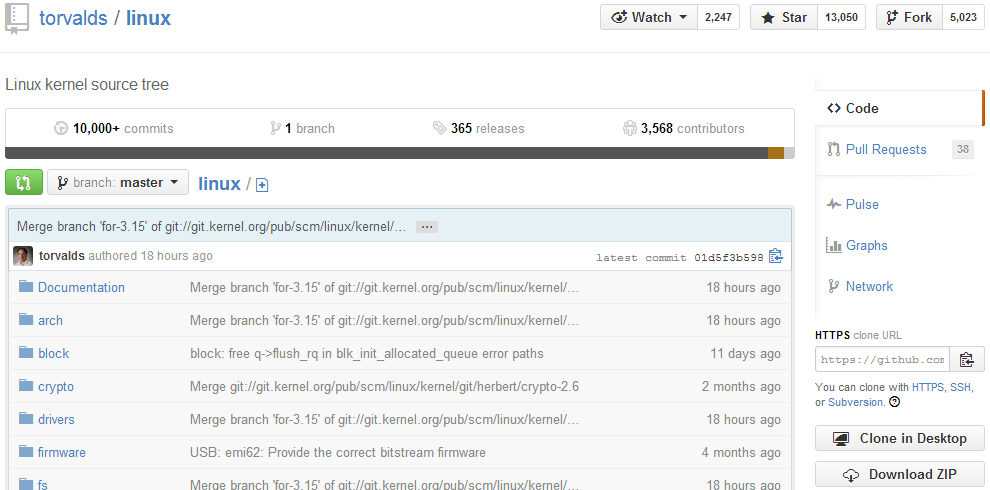
\includegraphics[width=0.98\textwidth]{./img/linux.png}
	\caption{Sample profile of a repository in GitHub}
	\label{fig:ghrepo}
\end{figure*}
With the advent of Web 2.0, online collaboration has become not only a part of internet experience but rather a necessity. People today are not just passive viewers of content but rather active contributors. Social networking sites such as Facebook and LinkedIn allow users to create both their personal and professional identities, respectively. Further, online communities such as blogs and wikis allow people to express opinions, carry out discussions, ask questions and answer queries, among other things. In addition, media sharing and hosting websites such as YouTube ensure fast propagation and easy accessibility of digital content.

Clearly, digital collaborations have revolutionized the way information is generated (i.e. through multiple sources), stored (social graphs and complex data types) and accessed (fast and ubiquitous) using just a web browser. This is also true for software development. Recently, platforms such as SourceForge, GitHub, BitBucket and CodePlex have experienced a rise in popularity. They are also referred to as social coding platforms i.e. development environment that encourages formal and informal collaboration on software projects providing opportunities for discussion and sharing. Open Source Software (OSS) in particular has experienced a rise in popularity. These open source projects are licensed to be freely modified and distributed and hence are often developed publicly where multiple developers collaborate to add or modify functionality.

The social aspects of OSS development provides insight into the dynamics of collaborations and opens interesting opportunities for research. Several studies throw light on what drives people towards OSS. Some of these factors include personal need for software \cite{Raymond1999}, creative stimulation \cite{lakhani2005}, learning \cite{Lakhani2003}, gift-giving intentions \cite{Zeitlyn2003} and significant returns on contribution \cite{ghosh2005}. Even though the developers have these intentions in mind, they seldom have any explicit metric to measure such factors. In the absence of such information developers indirectly assess the reputation of a project or a developer based on several other factors. For instance, number of followers of a developer can be indicative of their reputation in the coding community.

In this paper we will focus on collaborations between software developers, ``Social Coding'' and OSS development. We will discuss how these collaborations function by analysing one of the most popular social coding website - GitHub \cite{GitHub}. We are particularly interested in studying what motivates a developer to contribute into a project. The large amount of projects that a developer can join and contribute seems overwhelming. Yet, somehow, some of the projects seem to be more attractive to developers and have larger communities that are willing to  contribute to their development. A simple intuition of this phenomenon would be that popular projects attract developers simply because they are popular, like a snowball effect.

While this might be true for some projects, various counterexamples can be found in which a project quickly gathers a significant following, with no obvious reason. Our study will focus on analyzing the social network of GitHub and provide some answers to the following questions:

\textbf{Q1:} What is a typical contributor of a project?

\textbf{Q2:} Why do people follow specific projects?

We believe that by answering these questions we can help developers build a following to their projects. The remainder of our paper is structured as follows: In section 2 we will discuss similar factors that can affect collaboration decisions and reputation by reviewing some of the previous work that has been done in the field. Section 3 presents the data collected from Github and use it to answer Q1. In section 4, we analyze some trends on the data and use them to answer Q2. In section 5, we discuss some threats to the validity of our work. Finally, in section 6 we present our conclusions.


\section{Related Work}
\label{sec:related}

\cite{Thung2013} investigates the network structure of social coding in GitHub. In this study, they try to measure the strength of a) relationships among different projects and b) relationship between the developers. For this, they create network graphs of 30,000 projects randomly sampled from a set of 1,00,000 projects returned by the GitHub API and then randomly select 30,000 developers from these projects. This data is used to create two networks - A project-project network and a developer-developer network. In the project-project network each node of the network is a project and two projects are connected if they have at least one common developer. A weight is associated to each edge which signifies the number of developers that work on both the projects. In similar way the developer-developer network is constructed where nodes represent the developers and an edge is drawn between two developers when they work together on at least one project. Weight in this network represents the number of projects the two developers have worked upon together. These graphs are then analysed on three network characteristics - 1) Node degree 2) Network diameter and 3) Average shortest path using methodologies mentioned in \cite{Surian2010}. The authors also use the PageRank algorithm on these networks to find out the most influential projects and developers. The results show that the project networks are more interconnected than human networks and that social coding enables substantially more collaboration among developers.

In \cite{Dabbish2012}, the effect and value of ``transparency'' on people's inferences and decisions is analysed. This study is based on \cite{weiner2013}, in which it is claimed that ``awareness about the activities of user behavior on a social website enables other users on the network to draw inferences''. They performed a series of 24 semi-structured interviews with GitHub users where they were asked about the inferences they make about a user or a project and whether these inferences influence the projects or the people they follow. As expected, a rich set of inferences were made mostly based on 4 visual cues namely volume of activity, sequence of actions over time, attention to artifacts and people and the detail of information about an action. Each of these cues revealed a different type of information to the user making the inferences. For example, one of the users said that commits on a project revealed direction and intent of the contributor.


\section{Data Collection}
\label{sec:collection}
\begin{table}
\centering
\begin{tabular}{ | c | c | c | c | }
	\hline
	Users & Repositories & Followers & Followings \\ \hline
	Top 10 & 93.4 & 10,231.4 & 81.3 \\ \hline
	Top 100 & 129.1 & 3,203.2 & 70.6 \\ \hline
	Top 1K & 70.8 & 744.5 & 121.0 \\ \hline
	Top 10K & 45.8 & 147.7 & 49.2 \\ \hline
	All & 5.1 & 4.1 & 2.8 \\ \hline
\end{tabular}
\caption{Average repositories, followers and followings for GitHub users. Users are ordered by the number of followers. By Top 10 we mean the 10 most followed users. Same applies for Top 100, Top 1K and so on.}
\label{tbl:topusers}
\end{table}
\begin{table}
\centering
\begin{tabular}{ | c | c | c | c | }
	\hline
	Repos & Stars & Forks & Issues \\ \hline
	Top 10 & 21,564.0 & 5,972.8 & 306.1 \\ \hline
	Top 100 & 8,832.3 & 2,309.7 & 204.3 \\ \hline
	Top 1K & 2,600.1 & 622.2 & 141.0 \\ \hline
	Top 10K & 491.0 & 121.2 & 28.7 \\ \hline
	All & 8.5 & 2.2 & 0.6 \\ \hline
\end{tabular}
\caption{Average stars, forks and issues for GitHub repositories. By Top 10 we mean the 10 repositories that have the biggest number of stars. Same applies to Top 100, Top 1K and so on.}
\label{tbl:toprepos}
\end{table}
\begin{table}
\centering
\begin{tabular}{ | l | c | c | }
	\hline
	\multicolumn{1}{|c|}{Company} & Users in Top 10 & Users in Top 1K \\ \hline
	GitHub & 4 & 41 \\ \hline
	Google & 2 & 23 \\ \hline
	Khan Academy & 1 & 1 \\ \hline
	Linux Foundation & 1 & 1 \\ \hline
	Segment.io & 1 & 3 \\ \hline
	Basecamp & - & 4 \\ \hline
	Heroku & - & 7 \\ \hline
	Twitter & - & 11 \\ \hline
	Others & - & 556 \\ \hline
	Not Specified & 1 & 353 \\ \hline
\end{tabular}
\caption{Number of users that a company has between the Top 10 and Top 1K. It shows, for example, that 2 of the users working for Google are between the 10 most popular. This number grows to 23 when the 1K most popular users are considered.}
\label{tbl:topcompanies}
\end{table}

We used GitHub API v3 \cite{GitHubAPI} to collect the data. The advantages of such API is that it provides a more structured and straightforward access to the data. The disadvantage is that it only allows 5,000 queries per hour per user. An alternative to the API would be to create our own web crawler/scraper, with the risk of our IP getting banned by GitHub. We eventually found a way to paralelize the data collection phase, with the use of several user accounts. We built a tool that, given an initial set of users, would recursively fetch a random subset of his/her followers. For the initial set, we chose the one thousand most popular users, plus some chosen randomly. The same could not be done for the repositories. There is no unified criteria for selecting the most popular repositories: number of forks, number of contributors, number of watchers and so on. We ended up including a random set of repositories, ordered by different criteria.

We collected information of 618,353 users in GitHub. Regarding Q1, Table \ref{tbl:topusers} provides an overview of the typical user in GitHub. For comparison purposes, we decided to group the data by the ranking of the user. This shows, for example, that the average number of followers between the 10 most popular users is almost three times that of the Top 100 users. An interesting trend shown here is that the top users are also following a considerable amount of users, with the top 1K users following an average of 121 users, compared to the 2.8 followings that the average user has. We also collected information of 868,177 repositories. The averages are shown in Table \ref{tbl:toprepos}.

Finally, Table \ref{tbl:topcompanies} shows the companies that employ the most popular users in GitHub. It is interesting to note that the ten most popular users are mostly employed by well-known companies. It also shows that the number of independent users is considerable, with 35.3\% of the first 1,000 most popular users declaring themselves as working on their own or representing themselves.



\section{Results}
\begin{table}
\centering
\begin{tabular}{ | c | c | c | c | }
	\hline
	\multicolumn{2}{|c|}{Project} & \multicolumn{2}{|c|}{Owner} \\ \hline
	Ranking & Followers & Ranking & Followers \\ \hline
	1 & 30,229 & 111,278 & 2 \\ \hline
	2 & 28,594 & 193,670 & 0 \\ \hline
	3 & 24,682 & >1,000 & -  \\ \hline
	4 & 23,830 & 21 & 4,161 \\ \hline
	5 & 22,167 & 193,670 & 0 \\ \hline
	6 & 21,227 & 111,278 & 2 \\ \hline
	7 & 17,485 & 12 & 5,213 \\ \hline
	8 & 16,543 & >1,000 & - \\ \hline
	9 & 15,648 & 87 & 1,406 \\ \hline
	10 & 15,235 & 33,877 & 12 \\ \hline
\end{tabular}
\caption{Relation between followers of a project (stars) and followers of the owner of the project. }
\label{tbl:owner}
\end{table}
\label{sec:results}

To answer Q2, we formulated four hypothesis in an attempt to characterize the motivations behind developers following a project. The hypothesis are: (i) popularity grows because the owner of the project is popular; (ii) popularity grows because the number of popular contributors working on it; (iii) popularity is affected by the programming language; (iv) popularity is determined by the category that it belongs to. We now present the results obtained for each of the four hypothesis:

\subsection{Owner}

The owner of the project is the user who originally created and published it on GitHub. We hypothesize that the popularity of the owner influences the popularity of the project he/she owns. A relation was made between the number of stars of the project and the number of followers of the owner. We started by analyzing the behaviour of the 100 most popular projects and their owners, hoping to find a positive correlation. Table \ref{tbl:owner} shows no concrete evidence about the 10 most popular projects. We could not find information about some of the owners in our database (rows 3 and 8), thus we can only affirm that they are not between the 1,000 most popular users (see Section \ref{sec:collection} for details).

A more general case is shown in Figure \ref{fig:owner}. It can be seen that a large number of popular projects have owners with little following. Finally, for the complete set of projects included in our sample, the correlation between owners and projects is 0.01, using Pearson's correlation coefficient. Therefore, we conclude that there is no correlation at all between stars and followers.
\begin{figure}
	\centering
	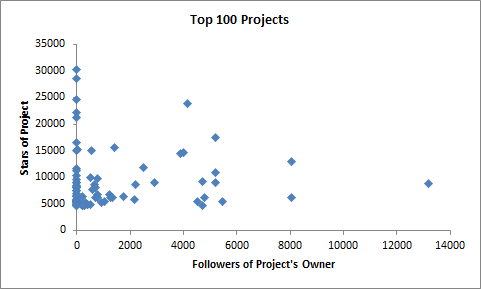
\includegraphics[width=0.45\textwidth]{./img/top100Owner.png}
	\caption{Relation between popularity of the project (given by stars) and the popularity of the project's owner (given by followers).}
	\label{fig:owner}
\end{figure}

\subsection{Contributors}

A contributor of a project is a user who actively participates in its development. We hypothesize that the involvement of one or more popular users on a project will influence on the project's popularity. In order to prove/disprove this, we collected the UserID of all contributors that belong to some of most popular projects. Due to the large amount of information and API restrictions, we could only collect the contributors of the one thousand most popular projects. We wanted to know how many popular users were contributing to such projects.

Table \ref{tbl:contributors} shows the relation between contributors and popularity of projects. We grouped the 100 and 1,000 most popular users and projects and determined the involvement of each. It shows, for example, that only 48 of the top 100 users are involved in the top 100 projects. Even more interesting, these 48 users are working on 18 of such projects. In other words, 82\% of the 100 most popular projects have no involvement of popular users. On the other side of the table, we have that almost a half (43\%) of the 1K most popular users are contributing to a quarter (22\%) of the 1K most popular projects. Because there's a large number of projects with no involvement of popular users, we dismiss this hypothesis as well.
\begin{table}
\centering
\begin{tabular}{ | l | c | c | c | c | }
	\hline
	\- & \multicolumn{2}{|c|}{Top 100 Projects} & \multicolumn{2}{|c|}{Top 1K Projects} \\ \hline
	\multicolumn{1}{|c|}{Users} & Uq Proj. & Uq Users & Uq Proj. & Uq Users \\ \hline
	Top 100 & 18 & 48 & 113 & 65 \\ \hline
	Top 1K & 23 & 286 & 222 & 431 \\ \hline
\end{tabular}
\caption{Relation between contributors and popularity of a project. Uq stands for Unique.}
\label{tbl:contributors}
\end{table}

\subsection{Programming language}

The programming language of a project can be a difficult choice for the owner. The owner probably wants to appeal to a broad audience by choosing a popular language. But sometimes there is no choice and the language is given by the specification of the project. For example, an Android app will have to be written with Java. For hypothesis 3, we wanted to determine the impact in popularity for choosing a specific programming language. We observed 128 different programming languages on our sample and a ``None'' language, which basically means that the project is missing that information. The metric we used for validating the hypothesis was the percentage of projects written in the same language that have more than 2,500 followers, a metric which we call the language success rate. We note that 2,500 followers is slightly lower than the average number of followers for the 1K most popular projects (See Table \ref{tbl:toprepos}), so we consider it a good popularity threshold.

The results are given in Table \ref{tbl:languages}. The total number of projects is given by P. F/P is the average number of followers per language and F > {$ \tau $} is the number of projects that have more than {$ \tau $} ({$ \tau $} = 2,500) followers. The last column is the language success rate. Several observations can be made. First, the two languages with the most projects (Javascript and Ruby) are also the ones that have the most projects above the {$ \tau $} threshold. Julia has a 50\% success rate, but its sample size is too little to make a reasonable generalization. Finally, the languages with a high average on followers are CSS, Rust, Julia and TypeScript, which are also the ones that have the highest success rate.

The correlation within the number of projects and the success rate is of 0.53, when the ``None'' language is removed. If we consider the ``None'' language, this correlation falls to 0.27. This tells us that there is some correlation between the most popular programming languages and the amount of projects that the language will have above the threshold {$ \tau $}. The only problem is that the success rates are so low or, in the case of Julia, the sample size is so little, that no positive conclusion can be made about the programming languages. So we also dismiss this hypothesis.
\begin{table}
\centering
\begin{tabular}{ | l | c | c | c | c | }
	\hline
	\multicolumn{1}{|c|}{Language} & P & F/P & F > {$ \tau $} & (F > {$ \tau $}) / P \\ \hline
	None & 171,894 & 1.89 & 3 & 0.002\% \\ \hline
	C & 39,716 & 8.55 & 15 & 0.038\% \\ \hline
	C\# & 15,240 & 7.84 & 1 & 0.007\% \\ \hline
	C++ & 26,071 & 7.49 & 5 & 0.019\% \\ \hline
	Clojure & 4,407 & 12.94 & 1 & 0.023\% \\ \hline
	CoffeeScript & 1,427 & 40.40 & 3 & 0.210\% \\ \hline
	CSS & 1,857 & 74.27 & 11 & 0.592\% \\ \hline
	Java & 57,953 & 6.76 & 11 & 0.019\% \\ \hline
	JavaScript & 106,987 & 17.40 & 107 & 0.100\% \\ \hline
	Julia & 2 & 1,780.00 & 1 & 50.000\% \\ \hline
	Objective-C & 20,784 & 21.87 & 21 & 0.101\% \\ \hline
	Perl & 43,808 & 2.72 & 1 & 0.002\% \\ \hline
	PHP & 54,337 & 8.39 & 12 & 0.022\% \\ \hline
	Python & 71,942 & 9.46 & 24 & 0.033\% \\ \hline
	Ruby & 173,960 & 8.89 & 51 & 0.029\% \\ \hline
	Rust & 62 & 76.18 & 1 & 1.613\% \\ \hline
	Shell & 14,158 & 9.68 & 7 & 0.049\% \\ \hline
	TypeScript & 92 & 99.39 & 1 & 1.087\% \\ \hline
	VimL & 13,961 & 9.31 & 8 & 0.057\% \\ \hline
\end{tabular}
\caption{Relation between programming languages and popularity of a project. The value chosen for {$ \tau $} was 2,500.}
\label{tbl:languages}
\end{table}
\subsection{Categories}
Our final hypothesis involves the categorization of projects. We claim that developers follow a project based on its intended usage. So, for example, 3D rendering software will usually have more followers than unit testing tools. We took the 100 most popular projects and visited their websites and repositories in order to find what their functionality is. We then assigned a broad category which we thought best described the project. The results are shown in Figure \ref{fig:categories}. We included the programming language as well, in order to better understand the distribution of the projects.

The most common categories are framework and widget / plugin. Examples of frameworks are JQuery and Symphony. Examples of widgets / plugins are FileUploader and JavaScript PDF reader. Also noteworthy to mention is that JavaScript frameworks and widgets / plugins are, by far, the most common types of project found on this phase of the study. Other categories found were front-end generators, libraries and networking tools. We believe this shows a trend about what kind of projects are users interested in following, i.e. web development productivity tools. This certainly shows the best results out of the four hypothesis we made. But, because the sample size is so small, we cannot generalize these results. In order to claim with some level of certainty that these categories correlate to the popularity of a project, we need to determine, out of all the frameworks hosted on GitHub, the percentage of successful ones. In other words, we suggest applying the same success rate metric we used for evaluating the programming languages.
\begin{figure*}[ht]
	\centering
	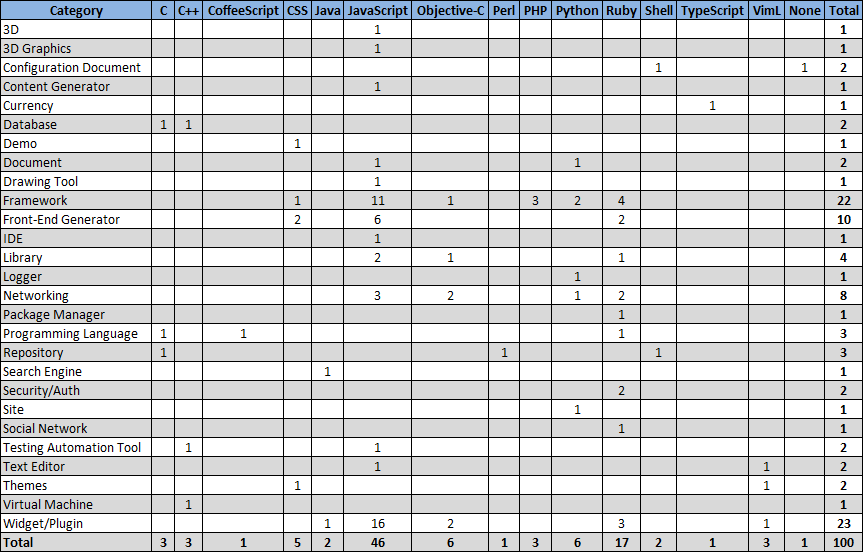
\includegraphics[width=\textwidth]{./img/categories.png}
	\caption{Categories of the 100 most popular projects, grouped by programming language. The most popular category is Widget/Plugin and 16 out of the 23 projects that fall within this category are developed using Javascript.}
	\label{fig:categories}
\end{figure*}


\section{Threats to Validity}
\label{sec:threats}

As stated on Section \ref{sec:collection}, we were able to collect only a fraction of the data that GitHub makes publicly available through their API. The limitation of 5,000 requests per hour per user, while generous, limited our progress. We believe that this is alleviated by the fact that our sample is of considerable size (20\% of the users and 10\% of the repositories). We also made sure we included the most popular users and repositories on our sample, by selecting them as a seed for our tool to recursively traverse the user/repository base of GitHub.

A major threat to our study is the influence of external factors as a driver for collaboration on users. Sites like \cite{SourceGraph} or \cite{OhLoh} act as search engines for open source projects and could potentially influence developers' contributions. These search engines use their own indexes and criteria to display results to users, possibly hiding the information of popularity of users and repositories. We believe that this is partially alleviated by the fact that these sites only work on a subset of the repositories. For example, in the case of \cite{SourceGraph}, they only index Python, Go, Ruby and Javascript repositories.

Finally, we were limited by the information provided by the GitHub API. As an example, we wanted to conduct an historical analysis on popular repositories and determine when did contributors join a repository, i.e. the date of a developer's first contribution. We hope this is solved on future releases of the API, but as of version 3.0, this feature is missing.


\section{Conclusions}

Scaling graph databases can be challenging, especially when dealing with highly
interconnected graphs.  We explored different, well-known caching algorithms
that allowed us to replicate data across partitions based on Zipfian read
workloads.  We also introduced a novel caching algorithm, Local Connected Cache
(LCC), as a way to exploit the underlying nature of graph data. LCC is a
multi-level LRU caching algorithm that assigns scores to vertices based on how
well connected they are to other local vertices on a given partition.

Although this algorithm highly favors immediate (1-hop) neighbours, we
showed that it does not perform well for k-hop neighbours and that is highly
dependent on the query access model that the underlying database implements.
We believe LCC will improve performance significantly if allowed to work with
intermediate caches, a direction we wish to pursue on future versions of the
platform.

We then compared two other caching algorithms, LRU and ARC, and showed
that ARC provides better performance in all three metrics that we collected.


\bibliographystyle{plain}
\bibliography{paper}
\end{document}
